\lecture[1]{Remotely Connected Electric Field\\ Generator}{lecture-text}

\subtitle{for Particle Separation in a Fluid}

\date{27 April 2016}


\begin{document}

\begin{frame}
  \maketitle
\end{frame}

\section{Dielectrophoresis}

% justin
\begin{frame}{Dielectrophoresis (DEP)}
  \begin{itemize}
  \item A dielectric particle in a non uniform 
  electric field experiences a force
  \item Different potential fields and frequencies 
  has an effect on the net force
  \item First studied in 1950s by Herbert Pohl
  \item Recently revived due to the ability to
  manipulate micro-particles and cells. 
  \end{itemize}
\end{frame}

% justin
\begin{frame}{Real World Application}
  \begin{itemize}
    \item Potential to separate particles in spinal fluid
    \item Act as filter
    \item Research in separating cancerous cells from healthy cells
    \item Separate platelets from whole blood
    \item Separate red and white blood cells
    \item Strains of bacteria and viruses
  \end{itemize}
\end{frame}

% tim
\section{Project Overview}

\begin{frame}{Project Description}
  \begin{itemize}
    \item A system to aid in the research of DEP
    \item Allow for quicker setup times
    \item Control Voltage and Frequency via the web
      \begin{itemize}
        \item 1 to 60 VPP
        \item 10k to 1Mhz
      \end{itemize}
    \item Hold output for long time periods
    \item Small Form Factor
    \item Easy to use
    \item Plug and play
  \end{itemize}
\end{frame}

\begin{frame}{Project Structure}
  \begin{itemize}
    \item Raspberry Pi
    \item Web Interface
    \item Web Server
    \item Frequency Control Solution
    \item Voltage Control Solution
  \end{itemize}
\end{frame}

\section{Initial Implementation}

\begin{frame}{Initial Implementation}
  \begin{block}{}
  \begin{itemize}
    \item Raspberry Pi 
      \begin{itemize}
        \item Host web server
        \item Remote manipulation of circuit output
        \item Web interface can provide additional functionality
        \item GPIO pins input to circuit
      \end{itemize}
    \item Circuit Output
      \begin{itemize}
        \item Frequency generated by GPIO pin 
        \item GPIO waveform integrated to get sine wave
        \item Sine wave amplified to form output
      \end{itemize}
    \end{itemize}
  \end{block}

  % \begin{center}
  % \includegraphics[width=1.0\textwidth,keepaspectratio]{Flowchar v1.jpg}
  % \end{center}
\end{frame}

\section{Intermediate Implementation 1}

\begin{frame}{Minigen Function Generator}
  \begin{itemize}
    \item SPI communications
    \item Small form factor
    \item Output to 
  \end{itemize}
\end{frame}

\begin{frame}{Intermediate Implementation}
  \begin{itemize}
    \item Raspberry Pi controls Integrated circuit components
    \item Produces frequency 10 Khz - 4 Mhz
    \item Digital Potentiometers
    \item SPI communications
    \item Vary resistance to control amplifier
    \item Amplifier controls voltage output from circuit
  \end{itemize}
\end{frame}

\begin{frame}{Problems and Setbacks}
  \begin{itemize}
    \item Mosfet Amplifier
    \item Digital Potentiometer
    \item Resistance drops with AC signal
    \item Distorted the sine wave
    \item Op Amps
    \item Slew Rates
    \item Gain Bandwidth
    \item Minigen
    \item B23 Bug
  \end{itemize}
\end{frame}

\begin{frame}{Digital Potentiometer Amplifier Circuit }
  \begin{itemize}
    \item "image"
  \end{itemize}
\end{frame}

\begin{frame}{MOSFET Amplifier}
  \begin{itemize}
    \item "picture"
    \item information
  \end{itemize}
\end{frame}

\begin{frame}{Problems and Setbacks}
  \begin{itemize}
    \item Lost a group member
    \item BJT Switch
    \item Control through GPIO pin
    \item Current Leaks through when logically off
    \item Relay
    \item Operating Frequency not sufficient
    \item Brandon
    \item We have had to make quite a few adjustments from our original plan.
    \item This is especially the case with our digital potentiometers.
  \end{itemize}
\end{frame}

\section{Intermediate Implementation 2}

\begin{frame}{SSR Circuit Implementation}
  \begin{itemize}
    \item "image"
  \end{itemize}
\end{frame}

\section{Final Design}

\begin{frame}{Overview}
\begin{block}{}
  \begin{itemize}
    \item Raspberry Pi controls integrated circuit components
    \item Minigen Function Generator
    \begin{itemize}
      \item SPI communications
      \item Produces frequency 10 Khz - 4 Mhz
    \end{itemize}
     \item Programmable Gain Amplifier(PGA)
    \begin{itemize}
      \item GPIO communications
      \item 8 voltage options (0-7)
    \end{itemize}
    \item Summing Amplifier
    \begin{itemize}
      \item Sums output from amplification stages
    \end{itemize}
  \end{itemize}
\end{block}
\end{frame}

\begin{frame}{Systems Diagram}
  \begin{center}
  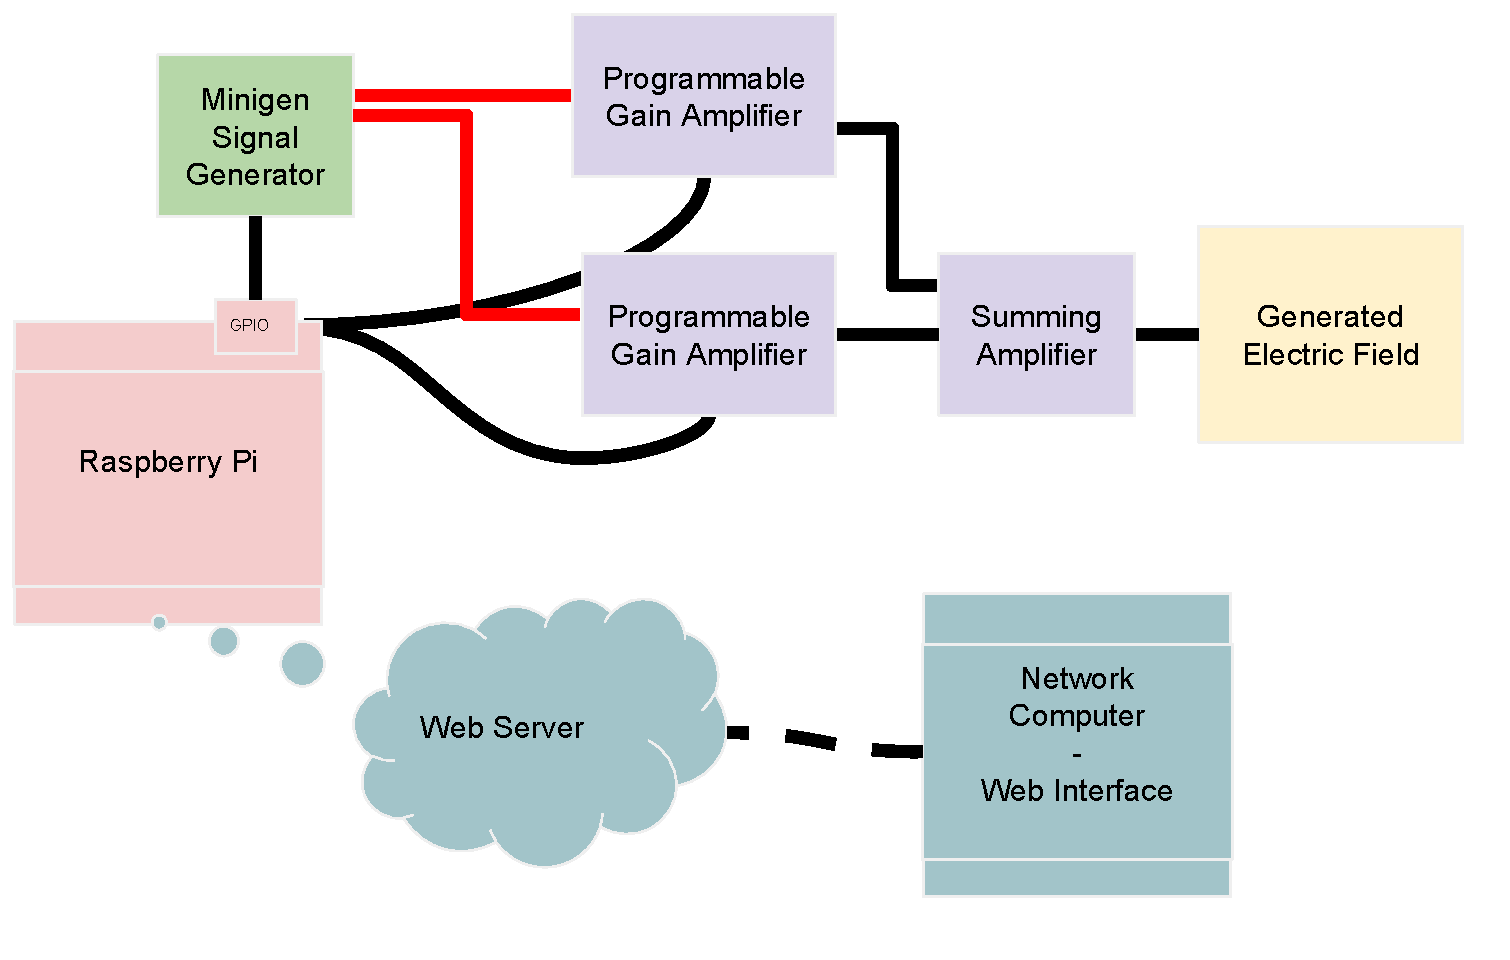
\includegraphics[width=1.0\textwidth,keepaspectratio]{block_diagram.pdf}
  \end{center}
\end{frame}

\begin{frame}{Amplifier Circuit}
  %\begin{block}{Components}
  \begin{itemize}
    \item Two stages with PGA and constant gain amplifiers
    \begin{itemize}
      \item Upper stage constant amplifier Gain 7.5 
      \item Lower stage constant amplifier Gain 1.07
      \item PGA's both having variable gain
    \end{itemize}
    \item Summing amplifier
  \end{itemize}
  %\end{block}

  \begin{center}
  \includegraphics[width=1.0\textwidth,keepaspectratio]{circuit_diagram.pdf}
  \end{center}
\end{frame}

% \begin{frame}{Computing Stage Gains}
%   \begin{itemize}
%     \item Hosted Locally
%   \end{itemize}
%     % voltage stage amplification computation
%     \begin{gather*}
%     A_1 = gain of stage 1 amp\\ 
%     A_2 = gain of stage 2 amp\\
%     A_{PGA} = max gain of PGA\\
%     V_{m1} = max voltage of stage 1\\
%     V_{m2} = max voltage of stage 2\\
%     V_{m1} + V_{m2} = 30V\\
%     V_{m1} = \frac{V_{m2}}{7}\\
%     V_{m1} + 7V_{m1} = 30V\\
%     8V_{m1} = 30V\\
%     V_{m1} = \frac{30V}{8}\\
%     V_{m1} = 3.75V\\
%     V_{m2} = 26.25V\\
%     A_{PGA} = 3.5V\\
%     A_1 = \frac{V_{m1}}{A_{PGA}} = \frac{V_{m1}}{3.5}\\
%     A_2 = \frac{V_{m2}}{A_{PGA}} = \frac{V_{m2}}{3.5}\\
%     A_1 = 1.07\frac{V}{V}\\
%     A_2 = 7.5\frac{V}{V}\\
%     \end{gather*}
% \end{frame}

\begin{frame}{Web Interface}
\begin{multicols}{2}
  \begin{itemize}
    \item Hosted Locally
    \item Able to be seen on intranet
    \item Voltage and Frequency controls
    \item Provides Additional Functionality
  \end{itemize}

\newpage

\begin{center}
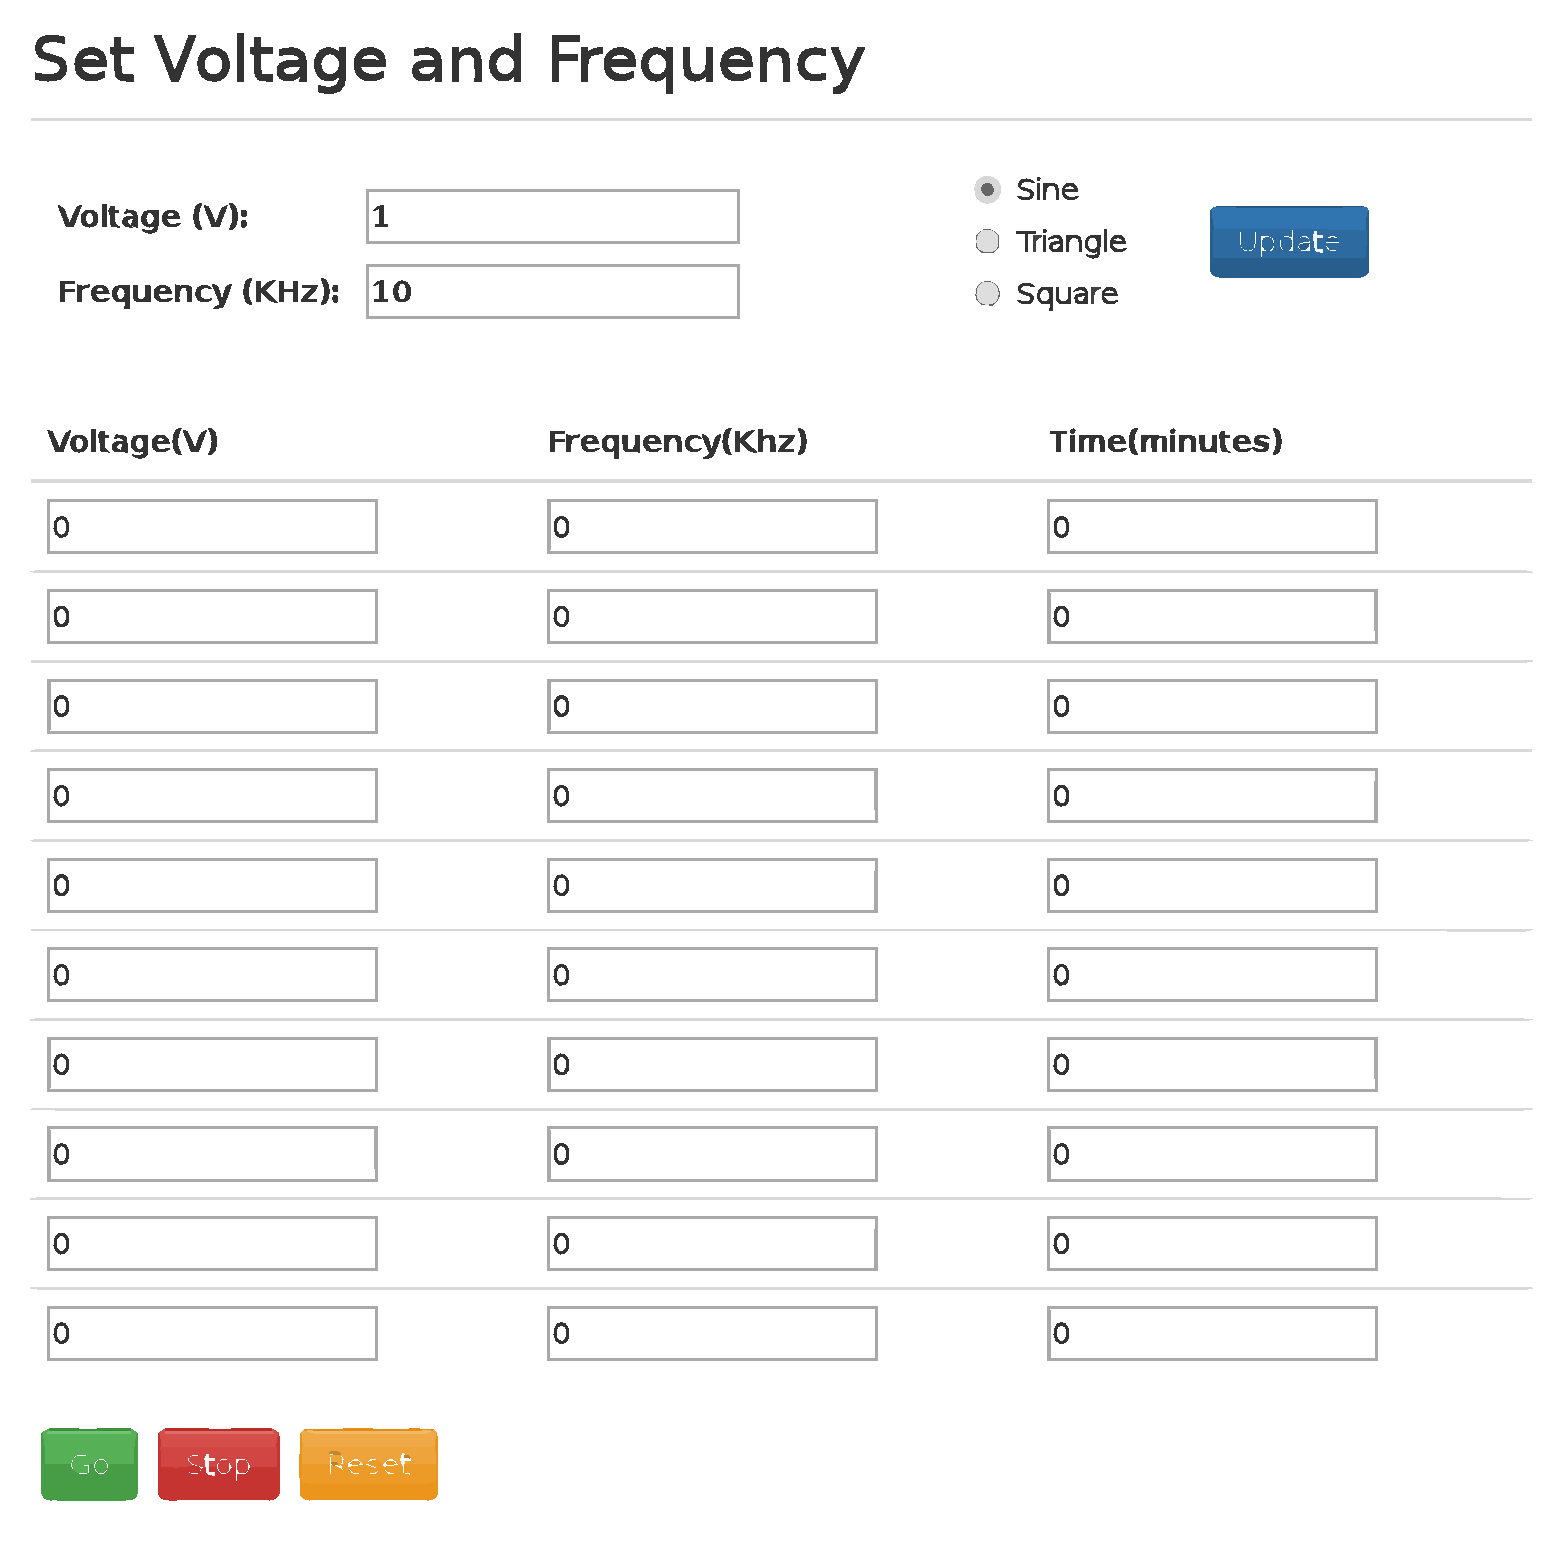
\includegraphics[width=0.5\textwidth,keepaspectratio]{web_interface.pdf}
\end{center}

\end{multicols}
\end{frame}

% talk about how the web interface accomplishes its job
\begin{frame}{Software Components}
\begin{multicols}{2}
  \begin{itemize}
    \item a
  \end{itemize}


\newpage

\begin{center}
\includegraphics[width=0.6\textwidth,keepaspectratio]{script_layout.pdf}
\end{center}

\end{multicols}
\end{frame}

% discuss the final state of the project
\section{Current State}

% discuss issues with the current state
\begin{frame}{Current State}
  \begin{block}{Problems}
    \begin{enumerate}
      \item Minigen B23 Bug
      \item Current op-amps have insufficient Gain-Bandwidth Product
        \begin{enumerate}
        \item Insufficient frequency
        \item Insufficient voltage
        \end{enumerate}
      \item Current draw from Raspberry Pi
    \end{enumerate}
  \end{block}

  \begin{block}{Solutions}
    \begin{enumerate}
      \item Most probably a hardware issue
      \item An op-amp with necessary specifications exists, 598-1449-ND
      \item Ensure few additional components connected to the Pi
    \end{enumerate}
  \end{block}
\end{frame}

\begin{frame}{Cost}
\begin{block}{Itemized Expenditures}
  \begin{center}
    \begin{tabularx}{1.0\textwidth}{|X|X|X|}
        \hline

        \textbf{Item} &
        \textbf{Quantity} &
        \textbf{Price(\$)} \\
        \hline

        \textbf{Raspberry Pi 3 Kit} &
        \textbf{1} &
        \textbf{49.99} \\
        \hline

        \textbf{Micro SD card} &
        \textbf{1} &
        \textbf{9.99} \\
        \hline

        \textbf{Minigen Function Generator} &
        \textbf{1} &
        \textbf{29.95} \\
        \hline

        \textbf{Op Amps} &
        \textbf{3} &
        \textbf{4.41} \\
        \hline

        \textbf{PGA} &
        \textbf{2} &
        \textbf{8.00} \\
        \hline

        \textbf{Miscellaneous Components} &
        \textbf{-} &
        \textbf{10.5} \\
        \hline

        \hline
        \textbf{Total} &
        \textbf{-} &
        \textbf{104.84} \\

        \hline
    \end{tabularx}
  \end{center}
\end{block}
\end{frame}

\begin{frame}{Logistical Setbacks}
\begin{block}{}
  \begin{itemize}
    \item Lack of manpower
    \item Loss of a team member at semester break
    \item Point of contact left company
  \end{itemize}
\end{block}
\end{frame}

\begin{frame}{Deliverables}
\begin{block}{} 
  \begin{itemize}
    \item Raspberry Pi loaded with controlling code
    \item User manual
    \item Current circuit implementation
    \item PCB design
    \item Simulation files
  \end{itemize}
\end{block}
\end{frame}

\section{Questions}

\begin{frame}{Questions?}
\begin{block}{Discussion Points}
  \begin{itemize}
    \item Dielectrophoresis (DEP)
    \item Circuit Design
    \item Digital Potentiometer/ Operation Amplifier
    \item MOSFET/ Programmable Gain Amplifiers (PGA)
    \item Web Interface
    \item Final Documentation
  \end{itemize}
\end{block}
\end{frame}

%
% extra slides for answering questions
%

\begin{frame}{Work Breakdown}
\begin{block}{Items}
  \begin{itemize}
    \item Initial Planning
    \item Project Website
    \item Reports and documentation
    \item Circuit Design
    \item Web Server
    \item SOC Communications
    \item PCB Design
  \end{itemize}
\end{block}
\end{frame}

\end{document}